\documentclass{beamer}
\usetheme{Boadilla}

\beamertemplatenavigationsymbolsempty

\usepackage[utf8]{inputenc}
\usepackage{caption, subcaption}
\usepackage{amssymb, amsmath, amsfonts}
\usepackage{graphicx}
\usepackage{xcolor}
\usepackage{appendixnumberbeamer}

\usepackage[square, numbers]{natbib}
\bibliographystyle{unsrt}

\DeclareMathOperator*{\argmin}{arg\,min}


\title[Data-driven targeted gene panels]{Data-driven design of targeted gene panels for estimating immunotherapy biomarkers}
\author[Bradley and Cannings]{Jacob R. Bradley, Timothy I. Cannings}
\date{January 2021}
% \institute[]{University of Edinburgh}


\titlegraphic{
\includegraphics[height=.7cm]{figures/mims_logo.png}\hspace*{.5cm}~%

\includegraphics[height=.7cm]{figures/uoe_logo.png}\hspace*{.5cm}~
   
\includegraphics[height=1cm]{figures/igmm_logo.png}
}

\begin{document}

\begin{frame}
\titlepage
\end{frame}

\begin{frame}{Abstract}
\begin{enumerate}[I]
    \item Problem: \textbf{Predict response to immunotherapy} with targeted gene panels.
    \item Our approach: First fit a \textbf{generative model} of exome-wide mutation, then use this to construct efficient \textbf{predictive models} of biomarkers such as \textbf{Tumour Mutation Burden (TMB)}.
    
\end{enumerate}
\end{frame}


\begin{frame}
\frametitle{Outline}
\tableofcontents
\end{frame}

\section{Biological/Clinical Background}


\subsection{Cancer and immunotherapy}
\begin{frame}{Cancer is a disease of the genome}
Cancer arises when DNA in cells changes (mutates) \citep{hanahan_hallmarks_2011}.
\begin{figure}[t!]
    \centering
    \begin{subfigure}[t]{0.45\textwidth}
        \centering
        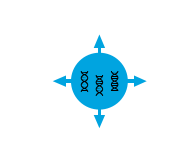
\includegraphics[height=1.5in]{figures/IC1.png}
        \caption{Non-cancer cell: Normal DNA.}
    \end{subfigure}
    ~ 
    \begin{subfigure}[t]{0.45\textwidth}
        \centering
        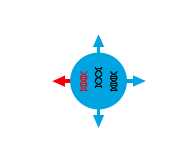
\includegraphics[height=1.5in]{figures/IC2.png}
        \caption{Cancer cell: Mutated DNA.}
    \end{subfigure}
\end{figure}
\end{frame}
\begin{frame}{Immunotherapy enables the immune system}
Immunotherapy 'releases the brakes' on the immune system in order for it to attack tumours \citep{pardoll_blockade_2012}.
\begin{figure}[t!]
    \centering
    \begin{subfigure}[t]{0.45\textwidth}
        \centering
        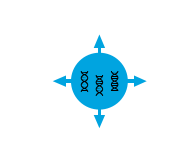
\includegraphics[height=1.5in]{figures/IC1.png}
        \caption{Low-damage cell: \textbf{unrecognisable} to immune system.}
    \end{subfigure}
    ~ 
    \begin{subfigure}[t]{0.45\textwidth}
        \centering
        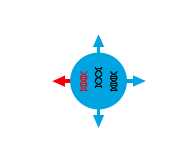
\includegraphics[height=1.5in]{figures/IC2.png}
        \caption{High-damage cell: \textbf{recognisable} to the immune system.}
    \end{subfigure}
\end{figure}
However, the immune system can only attack tumours that it recognises!
\end{frame}

\subsection{Exome-wide biomarkers}


\begin{frame}{Tumour mutation burden stratifies patients for immunotherapy response}
As a simple proxy for likelihood of immune response, we can use \textbf{tumour mutation burden}: the total count of non-synonymous mutations throughout the tumour exome \citep{zhu_association_2019, cao_high_2019}. \\
~\\
Advantages:
\begin{enumerate}[I]
    \item Calculated from DNA sequencing only (compatible with liquid biopsy \citep{gandara_blood-based_2018}).
    \item Relevant across cancer types.
\end{enumerate}
Disadvantages:
\begin{enumerate}[I]
    \item Requires Whole-Exome Sequencing (WES) to measure directly. 
    \item Fails to incorporate other features of the immune environment.
\end{enumerate}



\end{frame}

\subsection{Targeted gene panels}

\begin{frame}{Targeted panels make genomic biomarkers viable}
Rather than the entire exome/genome, targeted gene panels sequence a \textbf{subset} of genes.

\begin{figure}[t!]
    \centering
    \begin{subfigure}[t]{0.45\textwidth}
        \centering
        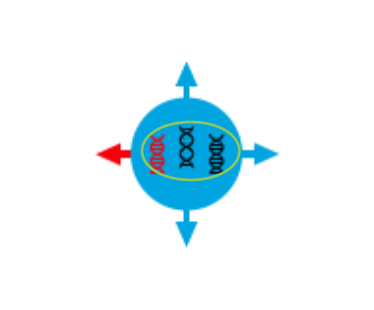
\includegraphics[height=1.5in]{figures/IC5.png}
        \caption{Whole-exome sequencing: \textbf{all genes} sequenced.}
    \end{subfigure}
    ~ 
    \begin{subfigure}[t]{0.45\textwidth}
        \centering
        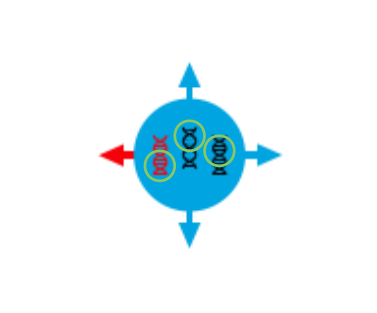
\includegraphics[height=1.5in]{figures/IC6.png}
        \caption{Targeted panel sequencing: \textbf{subset} of genes sequenced.}
    \end{subfigure}
\end{figure}

\end{frame}
\begin{frame}{Problem Statement}
Aims: 

\begin{enumerate}[1]
\item Select a discrete set of genes to form a panel (of pre-specified cost). 
\item Estimate TMB from panel sequencing data.
\end{enumerate} 
~\\
\end{frame}

\begin{frame}{Mutations and biomarkers: some notation}
We'll use $i,g,$ and $s$ to refer to:
\begin{enumerate}
    \item A sample $i$ (ranging from $i=1$ to $i=N$),
    \item A gene $g$ (belonging to some index set $G$),
    \item A variant type $s$ (for example synonymous/non-synonymous).
\end{enumerate}
Finally, we write:
\begin{enumerate}[4]  
    \item $M_{igs}$, to refer to a mutation count of a particular sample, gene, and mutation type.
\end{enumerate} 
~\\
We then can define the TMB of the $i$th sample via:
\[
T_i = \sum_{\substack{g \in G \\ s: \ \text{non-}\\ \text{synonymous}}} M_{igs}.
\]

\end{frame}

\section{Generative/predictive modelling framework}
\subsection{Generative model}

\begin{frame}{Our generative model}
A generative model of mutation attempts to capture the \textbf{underlying distribution} of variants across the entire exome/genome. \\
~\\
Our model incorporates \color{blue}\textbf{sample-specific} \color{black} effects, \color{red} \textbf{gene-specific} \color{black} effects, \color{green} \textbf{variant-specific} \color{black} effects, \color{purple} \textbf{variant-gene interactions} \color{black} and \color{cyan}\textbf{gene length}\color{black}:
\begin{equation}
    M_{igs} \sim \text{Poisson}(\phi_{igs})
\end{equation}
where 
\begin{equation}
\log(\phi_{igs}) = \color{blue}\mu_i \color{black}+ \color{red}\lambda_g \color{black} + \color{green} \nu_s \color{black} +  \color{purple} \eta_{gs} \color{black} + \color{cyan}\ell_g \color{black}
\end{equation} 
\end{frame}

\begin{frame}{NSCLC: Poisson-based generative model fit}
We fit our generative model with a WES non-small cell lung cancer dataset from Campbell et al. (2016) \citep{campbell_distinct_2016}.
\begin{figure}[htbp]
\centering
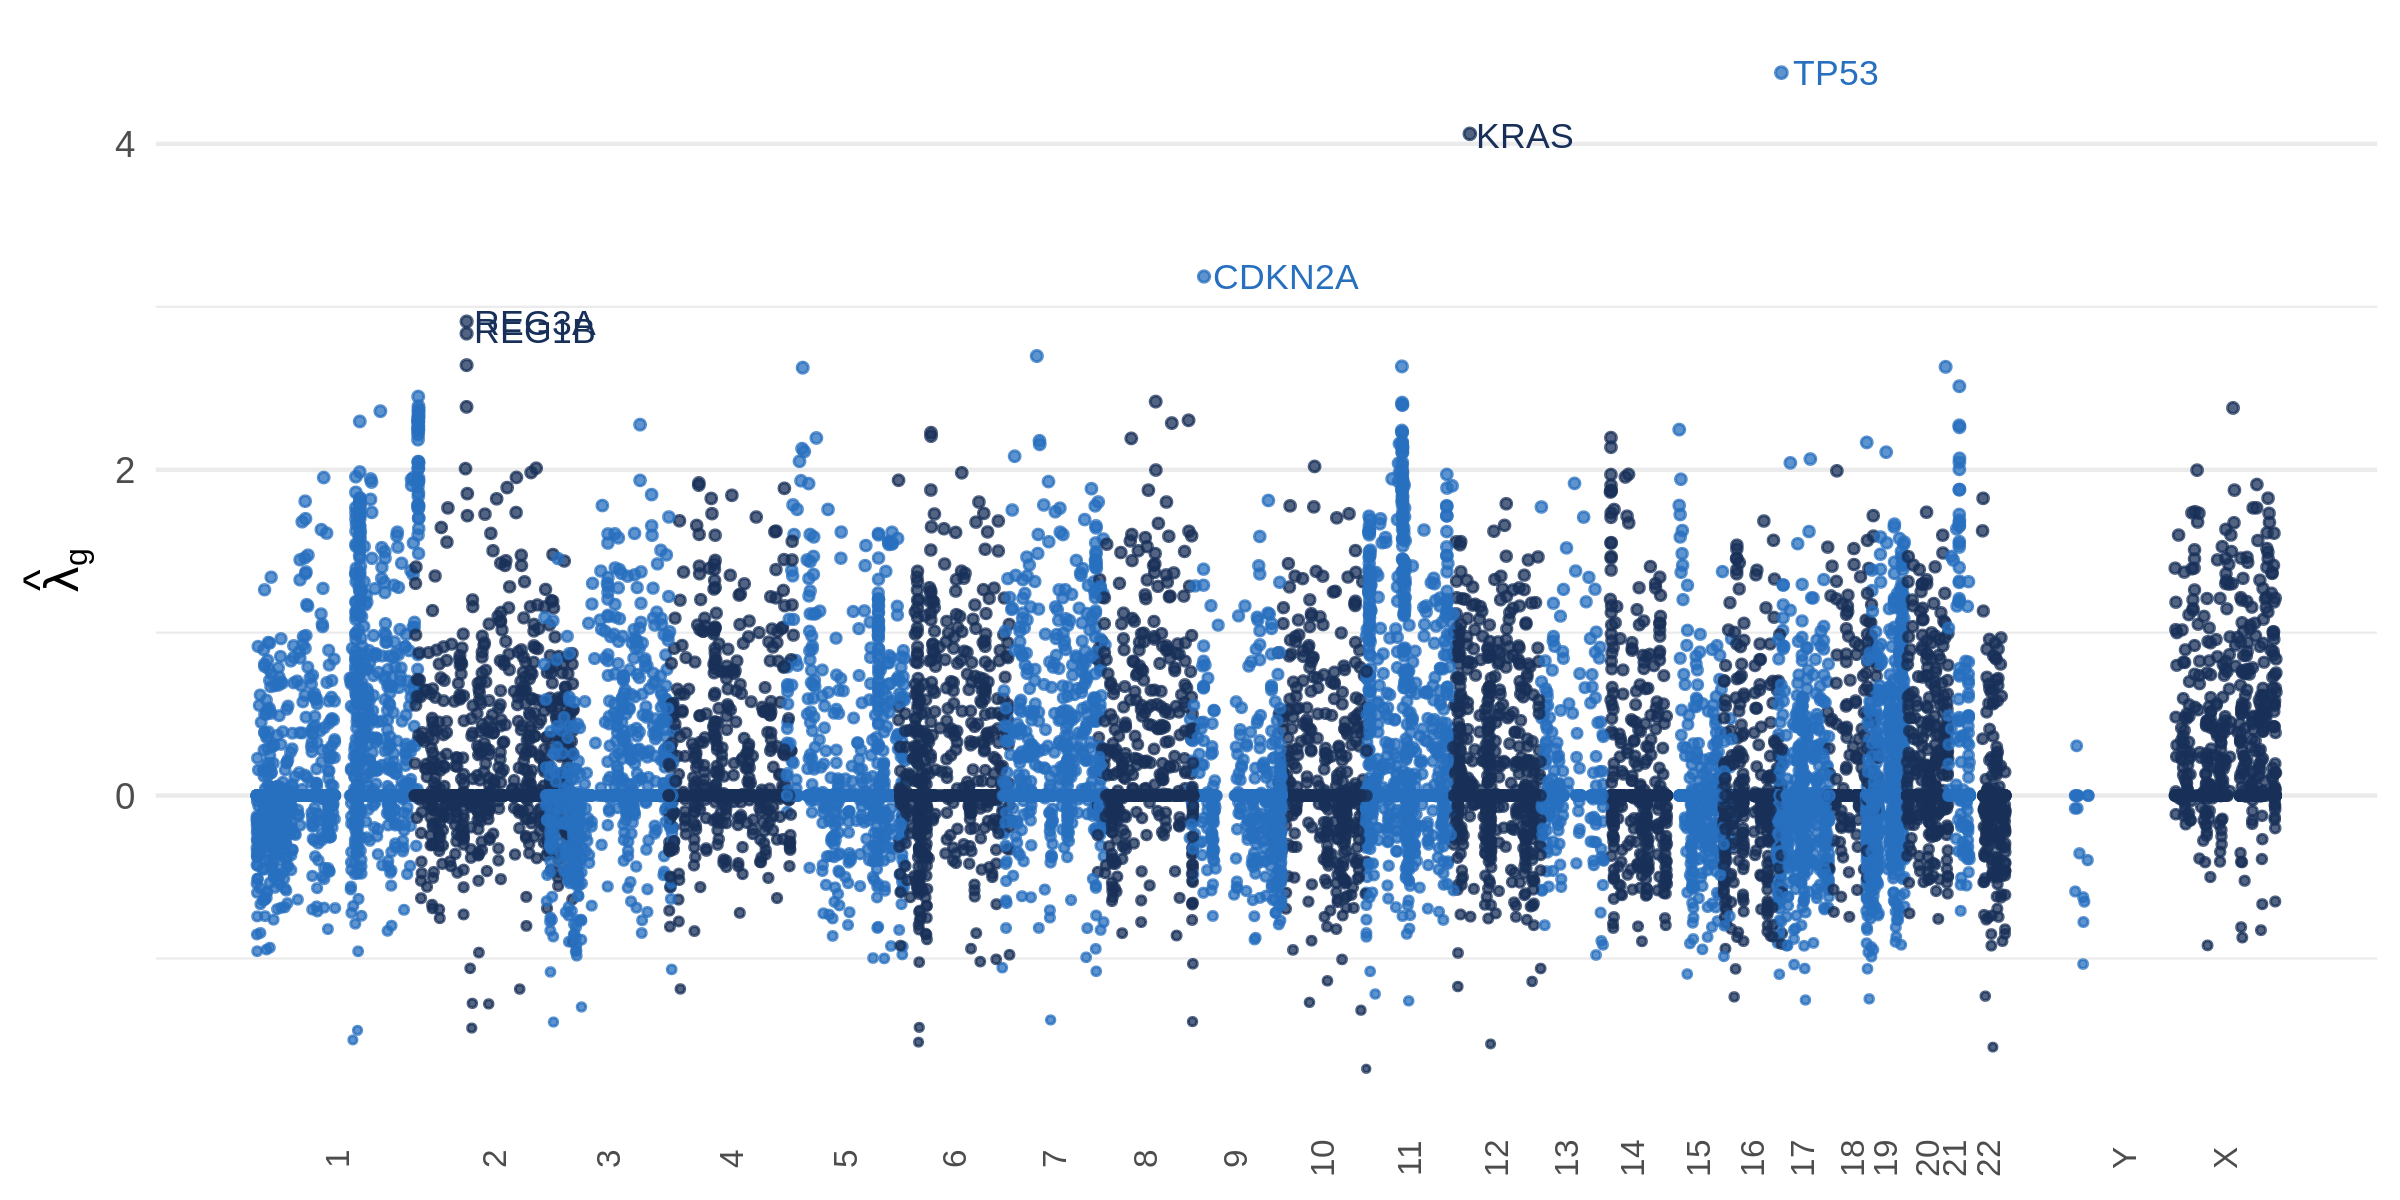
\includegraphics[width=4in]{figures/fig4.png}
\caption{Generative model parameters. \citep{bradley_data-driven_2021}\label{fig:3}}
\end{figure}
\end{frame}



\subsection{Predictive model}
\begin{frame}{Proposed estimator}
Aims (reminder): 

\begin{enumerate}[1]
\item Select a discrete set of genes to form a panel (of pre-specified cost). 
\item Estimate TMB from panel sequencing data.
\end{enumerate} 
~\\
Our estimator:

\begin{equation}
    \hat{T}_i(w) = \sum_{g,s} w_{gs} M_{igs}
\end{equation}

How we fit our estimator:
\begin{equation}
    \hat{w} := \argmin_w \bigg\{ \mathbb{E}\big[(\hat{T}_i(w) - T_i)^2\big] + \kappa |w| \bigg\} ,
\end{equation}
where $\kappa$ is a penalty specifying panel cost, and the expectation $\mathbb{E}$ is over the distribution learned by our generative model.
\end{frame}



\section{Application to non-small cell lung cancer}

\begin{frame}{NSCLC: Comparison panels and estimation methods}
We compare our methodology with four commercial gene panels, and with three other means of predicting TMB. These panels are:
\begin{enumerate}
\item The \color{red} TST-170 \color{black} gene panel.
\item The \color{green} Foundation~One \color{black} gene panel.
\item The \color{blue} MSK-IMPACT \color{black} gene panel.
\item The \color{purple} TSO-500 \color{black} gene panel.
\end{enumerate}
and these methods are:
\begin{enumerate}
    \item ecTMB  ($\times$) \citep{yao_ectmb_2020}.
    \item Simple counting ($\circ$).
    \item Linear regression ($+$).
\end{enumerate}

\end{frame}




\begin{frame}{NSCLC: Estimation performance}

\begin{figure}[htbp]
\centering
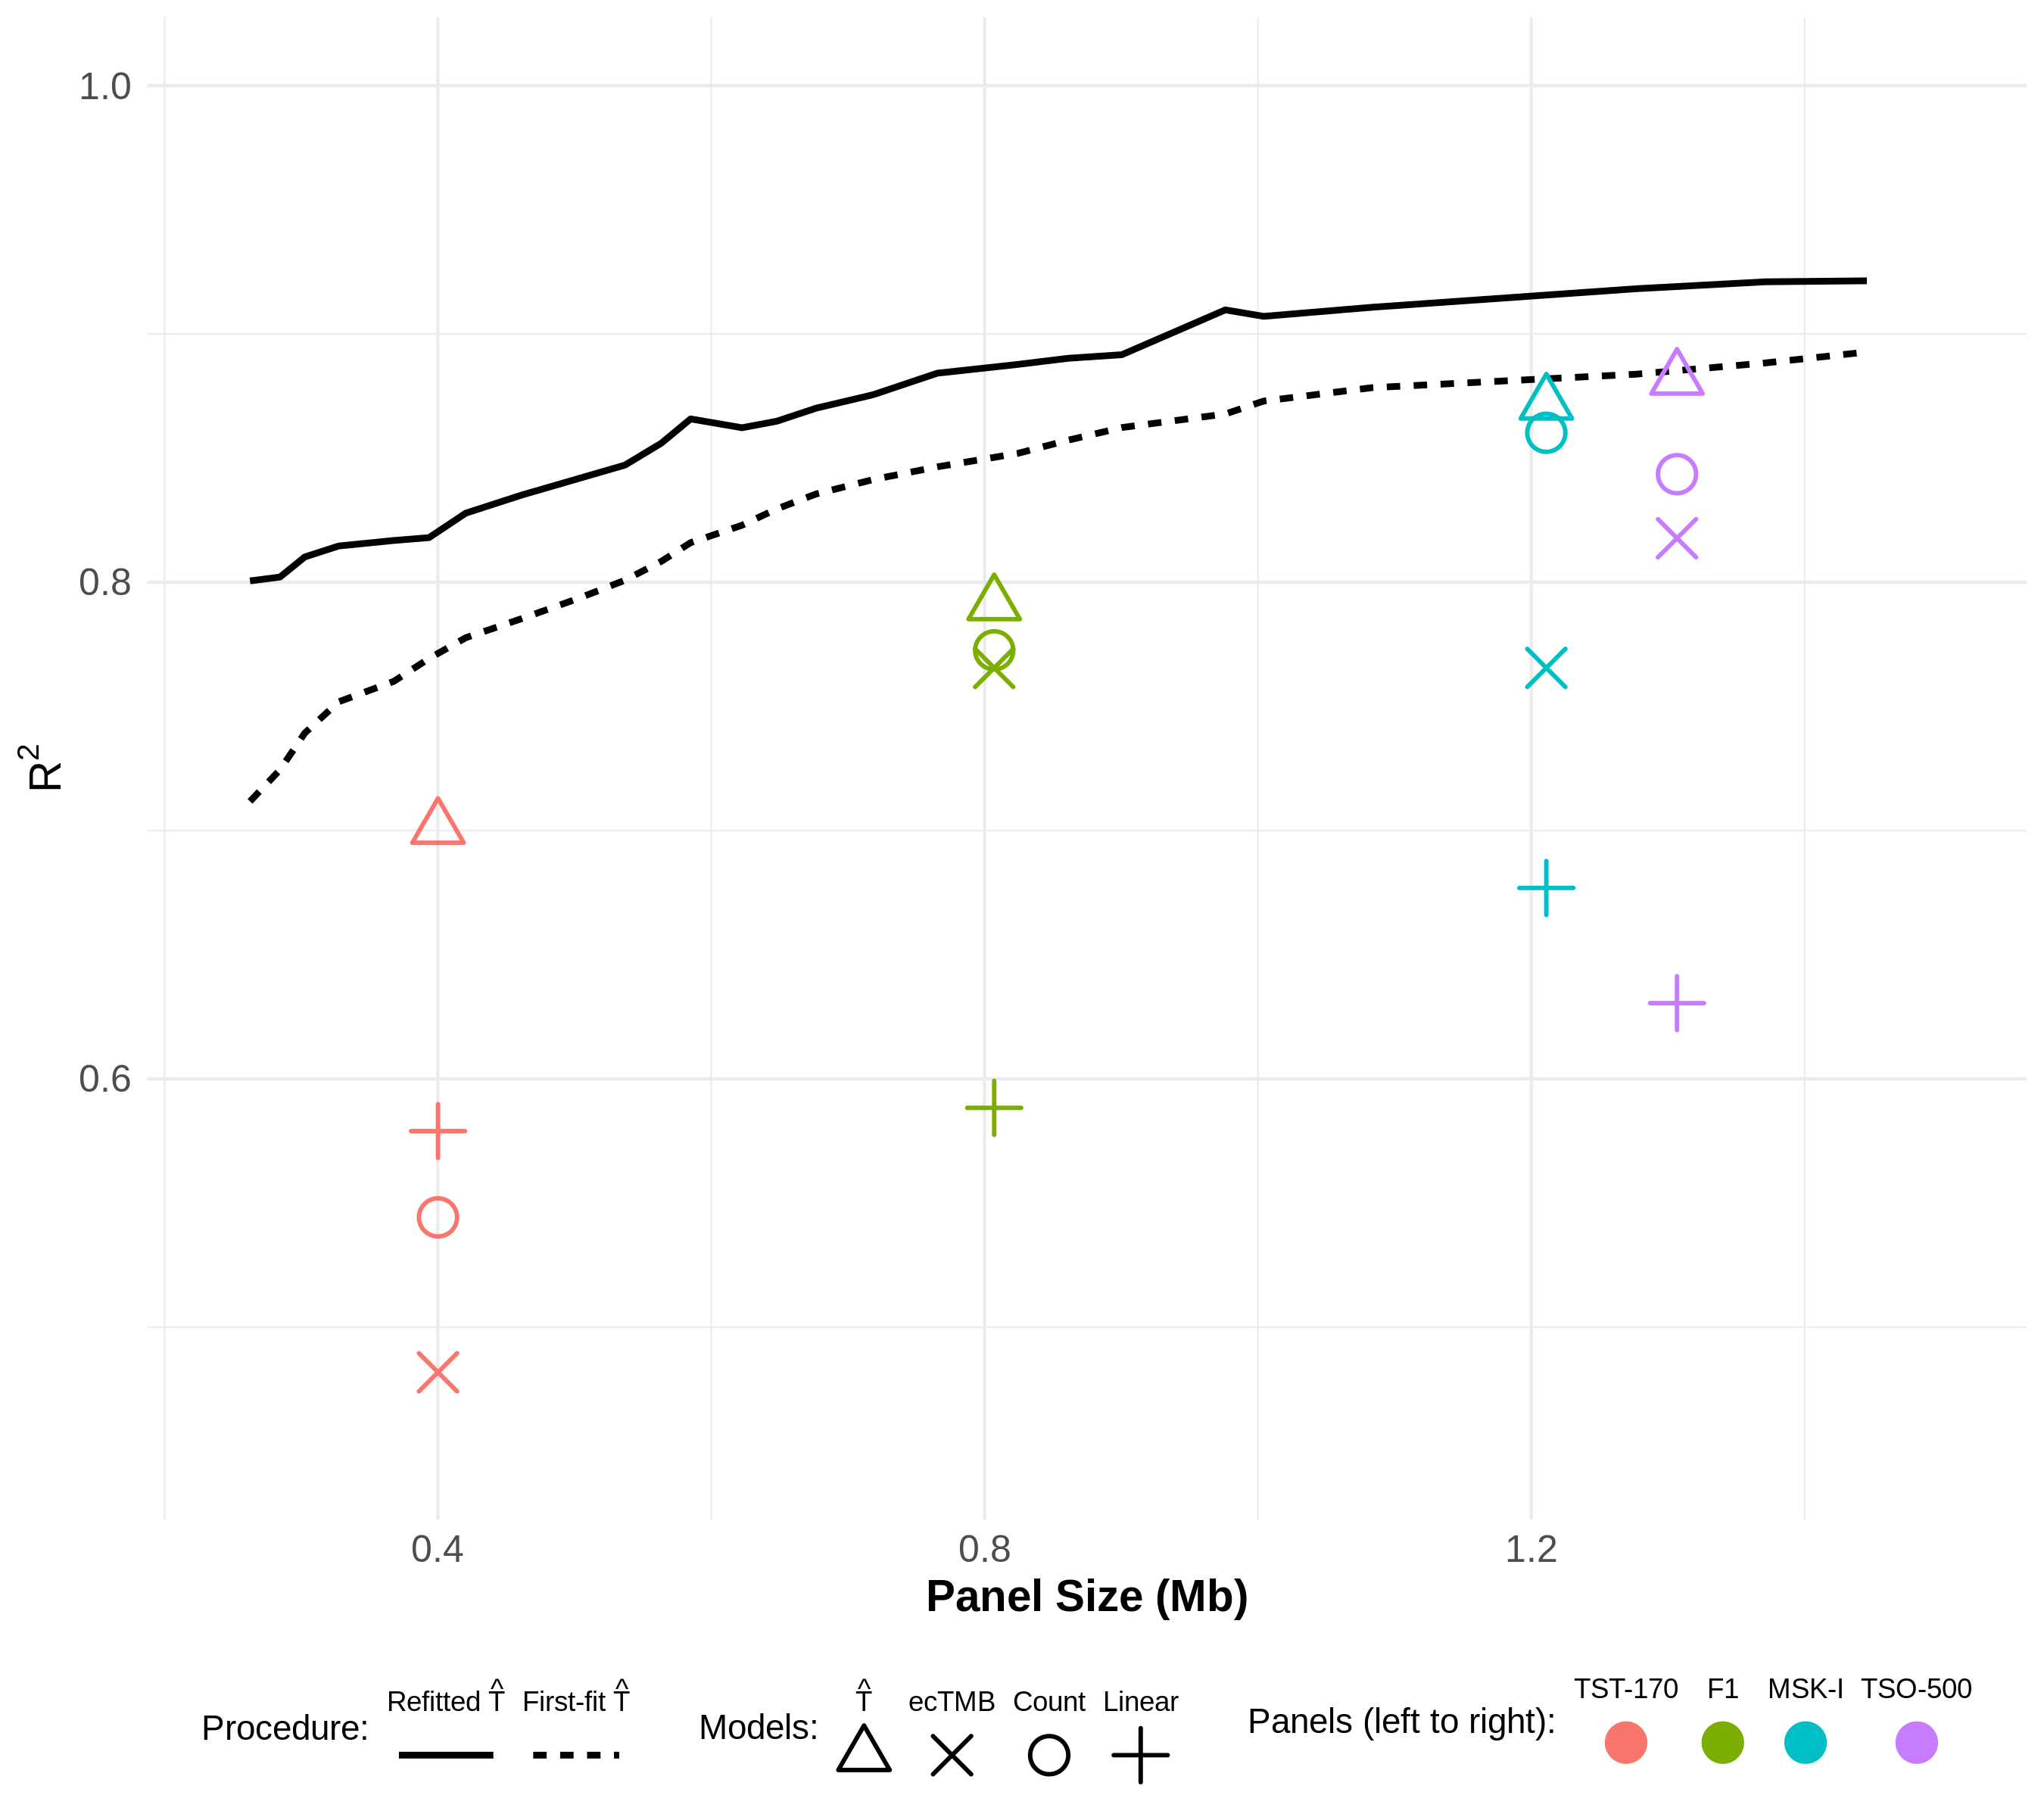
\includegraphics[width=3in]{figures/originalpanelcomparison.png}
\caption{Predictive model performance: comparison with commercial panels and other predictive methods \citep{bradley_data-driven_2021, yao_ectmb_2020}. \label{fig:7}}
\end{figure}
\end{frame}

\begin{frame}{Bonus material}
Our method is flexible enough that we can:
\begin{enumerate}
    \item Predict other exome-wide biomarkers, such as Tumour Indel Burden (TIB).
    \item Augment existing gene panels to improve their predictive performance.
\end{enumerate}
For more information check out our (draft) paper \cite{bradley_data-driven_2021}!
\end{frame}

\appendix
\begin{frame}[allowframebreaks]
        \frametitle{References}
        \bibliography{zotero-refs.bib}
\end{frame}

\end{document}